\renewcommand{\arraystretch}{.5}
\section{Grundformeln}
%\begin{longtable}{| m{.15\textwidth} | m{.15\textwidth} | m{.15\textwidth}|}%LAYOUT
%    \hline
%    &
%    \textbf{Formfaktor}&
%    \textbf{Crestfaktor}\\ \hline
%    
%    \tabbild[width=2cm]{images/GFSinus}&
%    \[ F=\dfrac{X_{RMS}}{|\overline{X}|} \]&
%    \[ C=\dfrac{\hat{X}}{X_{RMS}} \]\\ \hline
%    
%    \tabbild[width=2cm]{images/GFSinusSinus}&
%    \[ \sqrt{2} \]&
%    \[ \dfrac{\pi}{2 \sqrt{2}} = 1.11 \]\\ \hline
%    
%    \tabbild[width=2cm]{images/GFSinusGR}&
%    \[ 2 \]&
%    \[ \dfrac{\pi}{2} \]\\ \hline
%
%    \tabbild[width=2cm]{images/GFRechteck}&
%    \[ \sqrt{\dfrac{T}{\tau}} \]&
%    \[ \sqrt{\dfrac{T}{\tau}} \]\\ \hline
%    
%    \tabbild[width=2cm]{images/GFDreieck}&
%    \[ \sqrt{3} \]&
%    \[ \dfrac{2}{\sqrt{3}}=1.15 \]\\ \hline
%    
%\end{longtable}
\subsection{Leistungen}
\begin{minipage}{0.4\linewidth}
    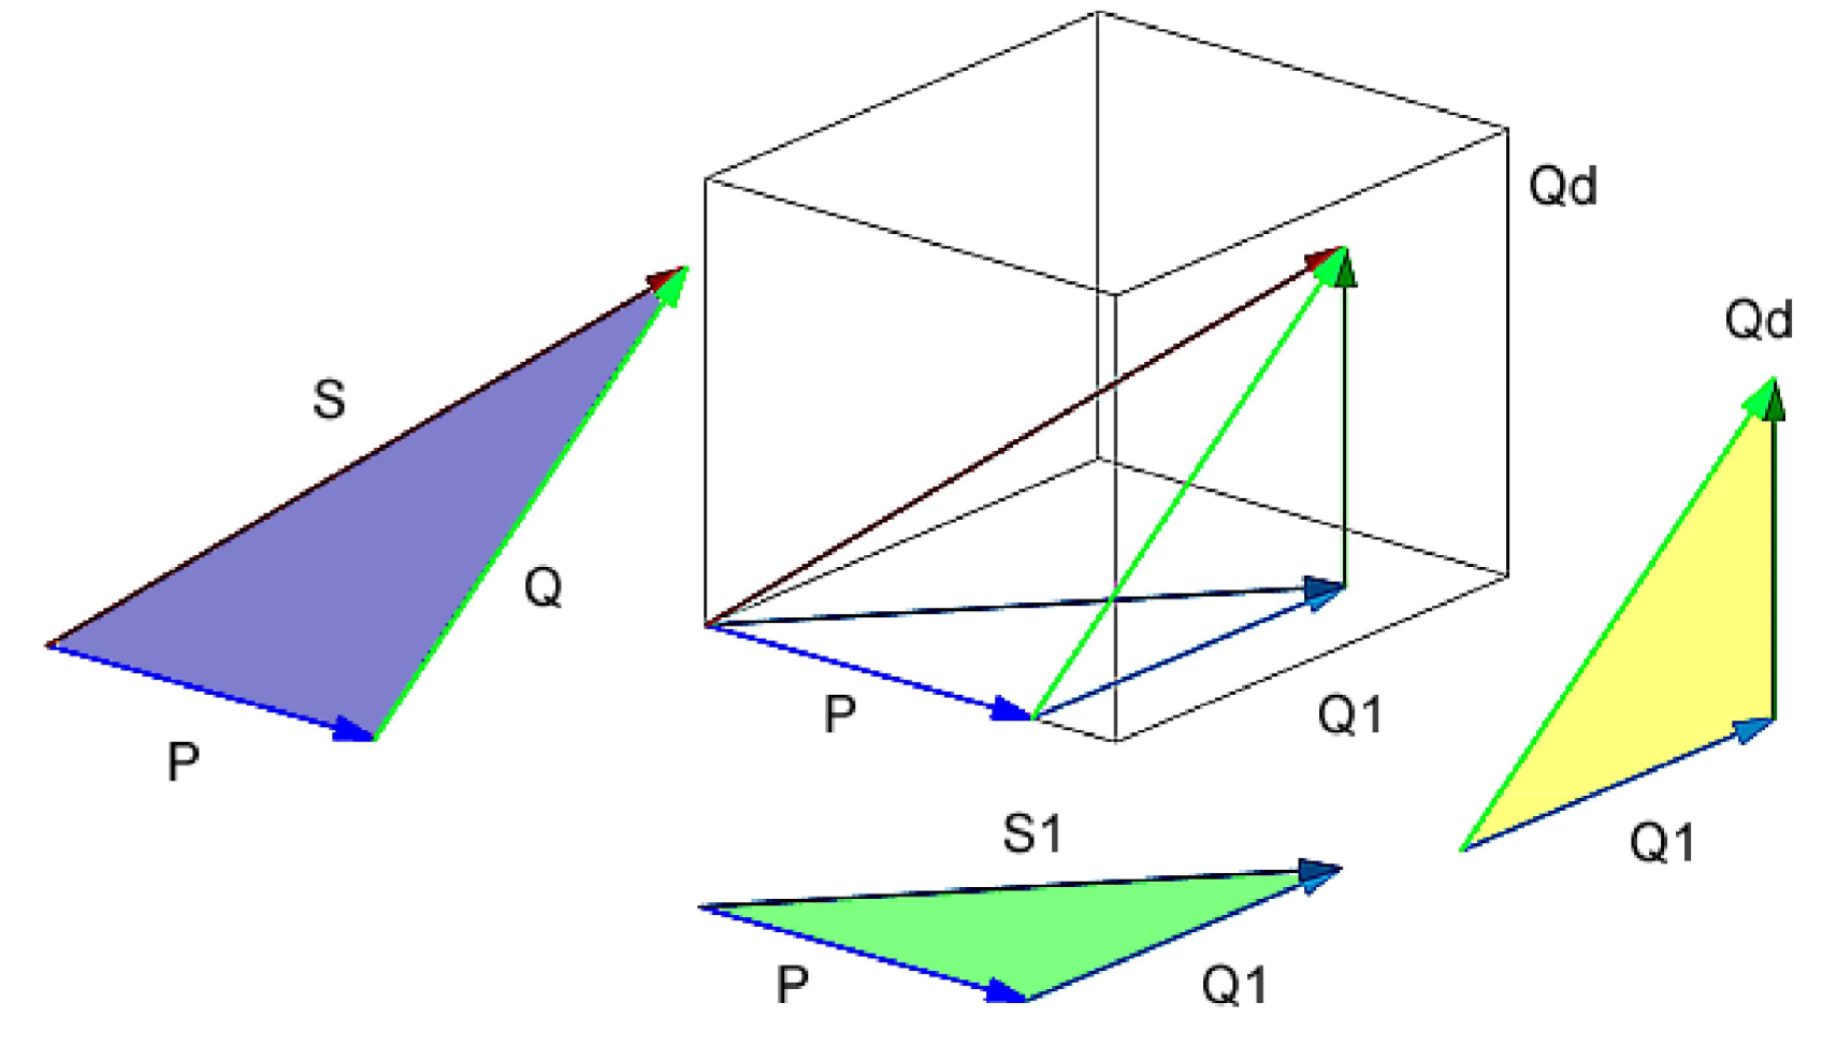
\includegraphics[width=\linewidth]{images/LeistungsDreieck}
\end{minipage}
\hspace{1cm}
\begin{minipage}{0.5\linewidth}
    Verzerrungsblindleistung entsteht, wenn $ I_1 $ und $ U_1 $ nicht in Phase sind. Wenn Oberwellen von Spannung und Strom die gleichen Frequenzanteile besitzen entsteht \newline keine Verzerrung.
\end{minipage}
\renewcommand{\arraystretch}{1.5}
\begin{longtable}{| p{.3\textwidth} | p{.40\textwidth} |p{.25\textwidth}|}
    \hline
    
    \textbf{{\color{blue}Scheinleistung}}&
    \vspace{-0.5cm}\[ S=U\cdot I =  \sqrt{P^2+Q^2} = \sqrt{P^2+Q_1^2+Q_d^2} \]\vspace{-0.5cm}&\textbf{i konjkolpex????}\newline V5S10 vs V7S14
    \\ \hline
    
    \textbf{Wirkleistung}&
    \vspace{-0.5cm}\[ P=U\cdot I_1 \cdot cos\varphi_1 \]\vspace{-0.5cm}&
    \\ 
    Wirkleistung (Trafoseitig)&
   \vspace{-0.5cm} \[ P = U_{RMS} \cdot I_{1\; RMS} \cdot sin(\varphi_1) \]\vspace{-0.5cm}&
    $ I_1 $= erste harmonische Komponente\newline
    $ \varphi_1 $= Phasenverschiebung
    \\\hline 
       
    \textbf{\color{yellow}Blindleistung}&
    \vspace{-0.5cm}\[ Q=U\cdot I_1 \cdot sin\varphi_1 = \sqrt{Q_1^2+Q_d^2} \]
    \[ Q_1 = S_1 \cdot sin \varphi_1 \]
    \[ Q_d = U\cdot \sqrt{\sum_{m=2}^{\infty}I_m^2}  = k \cdot S \]\vspace{-0.2cm}&
    $ Q_1 $= Grundschwingungs- \newline \quad Blindleistung\newline
    $ Q_d $= Verzerrungsleistung\newline
    \\ \hline
      
    \textbf{\color{green}Grundschwingungs-\newline scheinleistung}&
    \vspace{-0.5cm}\[ S_1=U_1\cdot I_1 = \sqrt{P^2+Q_1^2}\]\vspace{-0.5cm}&
    $ S_1 $= Grundschwingungs-Scheinleistung
    \\ \hline    
    \hline
    Berechnung des Mittelwertes&
    $X_{AV} = \frac{1}{T}\int\limits_{0}^{T}x(t)dt = \frac{1}{2\pi}\int\limits_{min}^{2\pi}\hat{U}_m\cdot sin(\beta)\diff \beta$
    &\\
    \hline
    Berechnung des Gleichwertes
    & $\overline{|X|} = \frac{1}{T} \int\limits_{0}^{T} |x(t)|dt$
    &\\
    \hline
    Berechnung des Effektivwertes
    & $X_{RMS} = \sqrt{\frac{1}{T}\int\limits_{0}^{T}x^2(t)dt}$
    &\\
    \hline
    Effektivwert Oberwellen
    & $X_{RMS\_Oberwellen} = \sqrt{X_{RMS}^2 - X_{AV}^2}$
    &\\
    \hline
    Formfaktor
    & $F = \frac{X_{RMS}}{\overline{|X|}}$
    &\\
    \hline
    Klirrfaktor
    &$ k= \dfrac{\sqrt{\sum_{k=2}^{\infty} I_k^2}}{\sqrt{\sum_{k=1}^{\infty} I_k^2}}$
    &\\
    \hline
    Welligkeit
    & $w = \frac{X_{RMS\_Oberwellen}}{|X_{AV}|}= \frac{\sqrt{\sum\limits_{k = 1}^{\infty}X_{k}^2}}{|X_{AV}|} = \sqrt{F^2-1}$
    &\\
    \hline
    Leistungsfaktor&
    $ \lambda = \frac{P}{S} = \dfrac{I_1}{I}cos\varphi_1 $
    & \\ \hline 
\end{longtable}
%========================================================
\clearpage
\subsection{Fourier}
\subsubsection{Allgemeine Form}
Eine periodische Funktion lässt sich durch eine Reihe von Sinus- und Kosinusfunktionen darstellen.
$$f(t) = \underbrace{\frac{a_{0}}{2}}_{\text{Gleichanteil}}+\underbrace{\sum_{k = 1}^{\infty} (a_{k} \cdot cos(k \omega t)+ b_{k} \cdot sin(k \omega t))}_{\text{Wechselanteil}} = f_{AV}+ \sum_{k = 1}^{\infty}\hspace{-1.3cm} \underbrace{c_k}_{\substack{\scriptsize \\[0.1cm]\text{Amplitude der Harmonischen}}}\hspace{-1.3cm} \cdot \sin(k\omega t + \varphi_k)$$

\begin{minipage}{0.5\linewidth}
    Die Koeffizienten der Entwicklung von $f(t)$ sind: \vfill
    \begin{tabular}{|ll|}
        \hline
        $a_{0} = \frac{2}{T}\int\limits_{0}^{T}f(t)dt$ & \\
        \hline
        $a_{k} = \frac{2}{T}\int\limits_{0}^{T}f(t) \cdot cos(k \omega t)dt$   &
         $(k = 0,1,2,...)$\\
        \hline
        $b_{k} = \frac{2}{T}\int\limits_{0}^{T}f(t) \cdot sin(k \omega t)dt$   &
         $(k = 1,2,3,...)$\\
        \hline
        $c_{k} = \sqrt{a_k^2 + b_k^2}$ &\\
        \hline
        $\varphi_k = \arctan(\frac{a_k}{b_k}) $&\\
        \hline
    \end{tabular}
\end{minipage}
\begin{minipage}{0.5\linewidth}
    \subsubsection{Orthogonalitätsbeziehungen}
    $\int\limits_0^T \cos(n\omega t)\cdot \cos(m\omega t)dt=
    \begin{cases}
    T,\ n=m=0\\
    \frac{T}{2},\ n=m>0\\ 
    0,\ n\neq m\\
    \end{cases}$\\
    
    
    $\int\limits_0^T \sin(n\omega t)\cdot \sin(m\omega t)dt=
    \begin{cases}
    \frac{T}{2},\ n=m\\
    0,\ n\neq m\\
    \end{cases}$\\
    $\int\limits_0^T \cos(n\omega t)\cdot \sin(m\omega t)dt=
    \begin{cases}
    0,\ \text{\footnotesize n-m=gerade Zahl}\\
    \dfrac{2m}{m^2-n^2},\ \text{{\footnotesize n-m=ungerade Zahl}}\\
    \end{cases}$
\end{minipage}

\begin{minipage}{0.5\linewidth}
\subsubsection{Komplexe Darstellung der Fourierreihen}
$$f(t) = \sum\limits_{k = -\infty}^{\infty} c_k \cdot e^{j k \omega t}$$ 
$$c_n=\overline{c_{-n}}=\frac{1}{T}\int\limits_0^T{f(t)\cdot e^{-jn\omega t}dt}$$
\end{minipage}
\begin{minipage}{0.5\linewidth}
\subsubsection{Umrechnungsformeln}
    $$c_n=\overline{c_{-n}}=\frac{a_n-jb_n}{2} (n=0,1,2,3,\ldots\text{ wobei }b_0=0)$$
    $$
    \left.
    \begin{array}{l} 
    a_n=2 \cdot \text{Re}(c_n)\\
    b_n=-2 \cdot \text{Im}(c_n)
    \end{array}
    \right\} 
    \quad
    (n=0,1,2,3,\ldots, b_0 = 0)$$
\end{minipage}
\subsubsection{Fourierreihe für beliebige Periode}
Gegeben: Periodische Funktion f mit \textbf{Periode L}\newline
\textbf{Reelle Fourierreihe}
\vspace{-0.3cm}
\begin{centering}
    $$ f(t) = \frac{a_0}{2} + \sum_{k=1}^{\infty}\left[a_k cos\left(\frac{2\pi}{L}kt\right)+b_k sin(\left(\frac{2\pi}{L}kt\right) \right] $$
\end{centering}
\vspace{-0.5cm}
\begin{multicols}{3}
{
    $  a_0 = \frac{1}{L} \int\limits_{0}^{L} f(\alpha) \diff \alpha $
    
    $  a_k =\frac{2}{L} \int\limits_{0}^{L}  f(\alpha) cos\left(\frac{2\pi}{L}k\alpha\right) \diff \alpha$
    
    $ b_k = \frac{2}{L} \int\limits_{0}^{L} f(\alpha) sin\left(\frac{2\pi}{L}k\alpha\right) \diff \alpha $
}
\end{multicols}
\subsubsection{Sätze zur Berechnung der Fourierkoeffizienten}
\textbf{Symmetrie}
\vspace{-0.2cm}
\begin{multicols}{2}
    \begin{minipage}{\linewidth}
        \textbf{Gerade $\quad f(t) = f(-t)$}\newline       
        Symetrisch an Y-Achse
        \[ b_{n} = 0, a_{n} = \frac{4}{T}\int\limits_{0}^{\frac{T}{2}} f(t) \cdot cos(n \omega t) \diff t \]      
        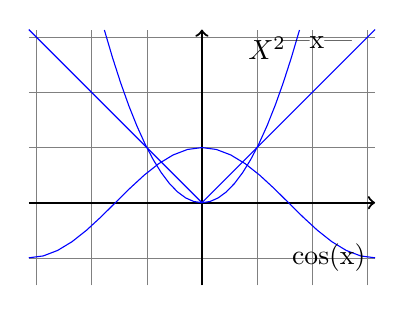
\begin{tikzpicture}[scale = 0.7]
            \draw [help lines] (-pi,-1.5) grid (pi,pi);  %Gitter
            \draw [thick, ->](-pi,0) -- (pi,0);          %x-achse
            \draw [thick, ->](0,-1.5) -- (0,pi);         %y-achse
            \draw [blue, domain=-1.77:1.77] plot (\x, {pow(\x, 2)});
            \node [left] at (1.7,2.8) {$ X^2$};
            \draw [blue, domain=-pi:pi] plot (\x, {cos(\x r)});
            \node [left] at (pi,-1) {cos(x)};
            \draw [blue, domain=-pi:pi] plot (\x, {abs(\x});
            \node [left] at (2.9,2.9) {|x|};
        \end{tikzpicture}
    \end{minipage}
                
    \begin{minipage}{\linewidth}
        \textbf{Ungerade $\qquad f(-t) = -f(t)$}\newline
        Punktsymetrisch am Ursprung
        \[  a_{n} = 0, b_{n} = \frac{4}{T}\int\limits_{0}^{\frac{T}{2}} f(t) \cdot sin(n \omega t)\diff t \]
        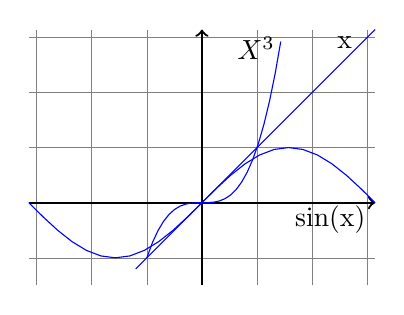
\begin{tikzpicture}[scale = 0.7]
            \draw [help lines] (-pi,-1.5) grid (pi,pi);  %Gitter
            \draw [thick, ->](-pi,0) -- (pi,0);         %x-achse
            \draw [thick, ->](0,-1.5) -- (0,pi);         %y-achse
            \draw [blue, domain=-1:1.43] plot (\x, {pow(\x, 3)});
            \node [left] at (1.5,2.8) {$ X^3$};
            \draw [blue, domain=-pi:pi] plot (\x, {sin(\x r)});
            \node [left] at (pi,-0.3) {sin(x)};
            \draw [blue, domain= -1.2:pi] plot (\x, {\x});
            \node [left] at (2.9,2.9) {x};
        \end{tikzpicture}
\end{minipage}
\end{multicols}
\clearpage